%mainmatter

\chapter{Vorwort}
%Preface

%\LR{
		%\subsection{sub1 Parallel} 
%		\blindtext 
%		}{
		%\esubsection{sub2 Parallel}
%		 \blindtext
%}

\chapter{Personal}
\echapter{STAFF}
%STAFF
%Emeritus
%Emrtitus
\section*{Emrtitus}
 
 \begin{minipage}[t]{\textwidth}
	\begingroup
	\parfillskip=0pt
	
  	\begin{minipage}[c]{0.25\textwidth}	
   		%\blindtext	
   		\centering
		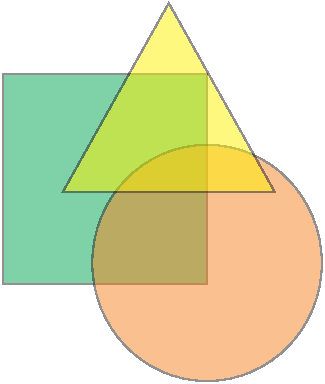
\includegraphics[width=0.7\textwidth]{Bilder/Grafik}		
		%\captionof{figure}{ Grafiken}	
			%\label{fig:GrafikOptionen}
  	\end{minipage}	
 	\hfill 	
  	\begin{minipage}[t]{0.7\textwidth}
  		\blindtext
  	\end{minipage}  
	\par\endgroup
\end{minipage}


% \begin{minipage}[t]{0.6\textwidth}
%	\begingroup
%	\parfillskip=0pt
%	% zwei weitere Minipages
%	\begin{minipage}[t]{0.47\textwidth}
%	\blindtext
%	\end{minipage}%
%	\hfill
%	\begin{minipage}[t]{0.47\textwidth}
%	\blindtext
%	\end{minipage}%
%	\par\endgroup
%\end{minipage}


%Technische Mitarbeiter und Sekretariat
%Technical staff and office
\newpage

\section*{Technische Mitarbeiter und Sekretariat}

\begin{figure}[htbp]
	% minipage mit (Blind-)Text
	\begin{minipage}[t]{0.18\textwidth} 
	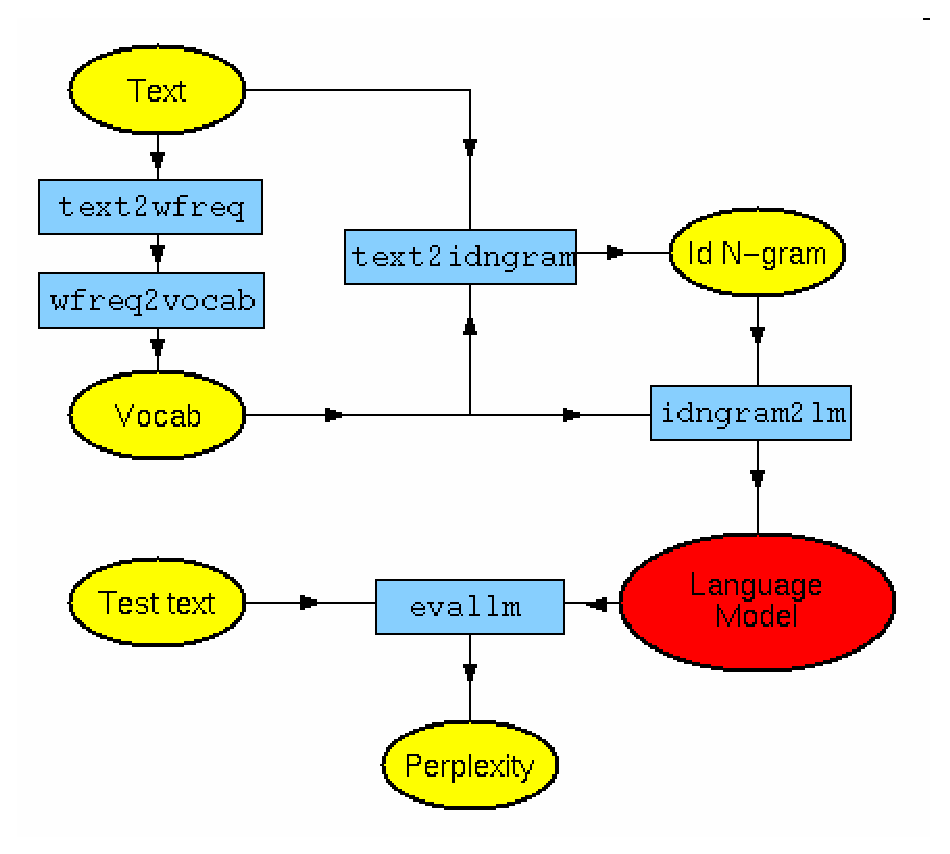
\includegraphics[width=\textwidth]{Bilder/toolkit.eps}
	%\caption{Eine Grafik}
	%\label{Bild}
	\end{minipage}
	% Auff�llen des Zwischenraums
	\hfill
	% minipage mit Grafik
	\begin{minipage}[b]{0.3\textwidth}
	% \textwidth bezieht sich nun auf die Minipage
 	\makebox[0.3\textwidth][l]{	\scriptsize{Dipl.-Ing Helmut Foth}	}\\
 	\makebox[0.3\textwidth][l]{	\scriptsize{Laboringenieur}	}\\
 	\makebox[0.3\textwidth][l]{	\scriptsize{Electrical engineering master}}\\
 	\makebox[0.3\textwidth][l]{	\scriptsize{Mitarbeit seit:1995}}\\		
 

 	
	% \caption{Der Text}
	% \label{Text}
	\end{minipage}
	\hfill
	% minipage mit (Blind-)Text
	\begin{minipage}[b]{0.18\textwidth} 
	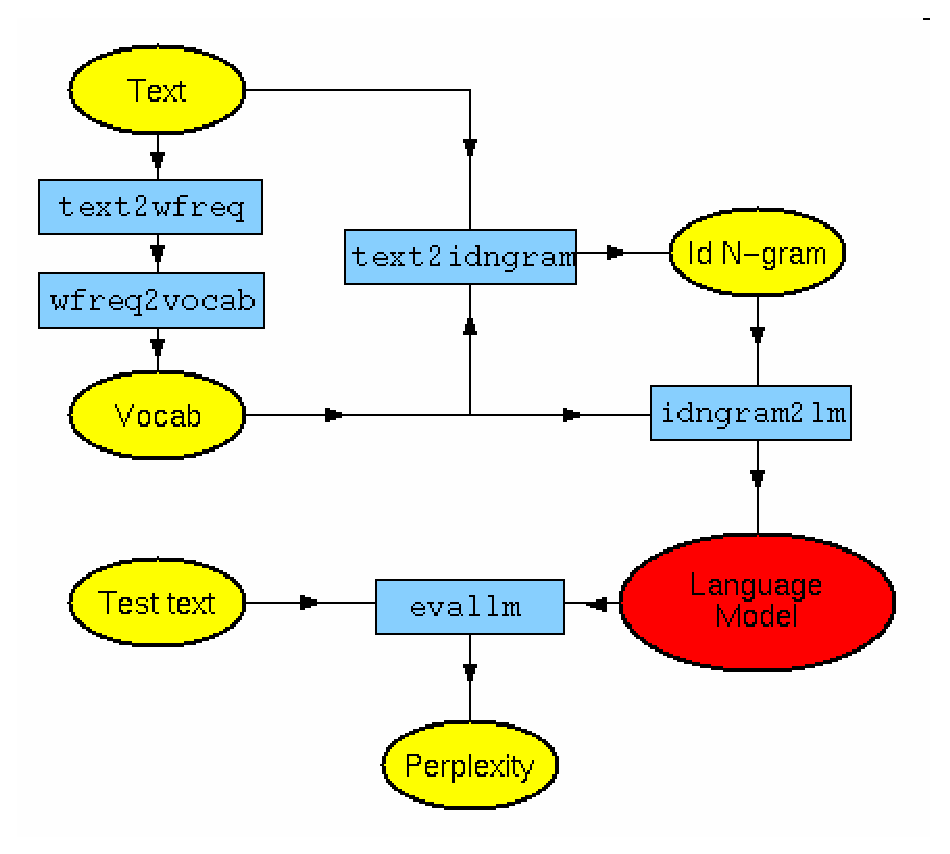
\includegraphics[width=\textwidth]{Bilder/toolkit.eps}
	%\caption{Eine Grafik}
	%\label{Bild}
	\end{minipage}
	% Auff�llen des Zwischenraums
	\hfill
	% minipage mit Grafik
	\begin{minipage}[b]{0.3\textwidth}
	% \textwidth bezieht sich nun auf die Minipage
 	\scriptsize{Title}\\
 	\parbox[b]{\textwidth}{
 	\scriptsize{Laboringenieur}	\\
 	\scriptsize{Electrical engineering technican}\\
 	\scriptsize{Mitarbeit seit:1995}\\	
 	}
	% \caption{Der Text}
	% \label{Text}
	\end{minipage}
% \caption{noch eine Caption}
\end{figure}


\begin{figure}[htbp]
	% minipage mit (Blind-)Text
	\begin{minipage}[b]{0.2\textwidth} 
	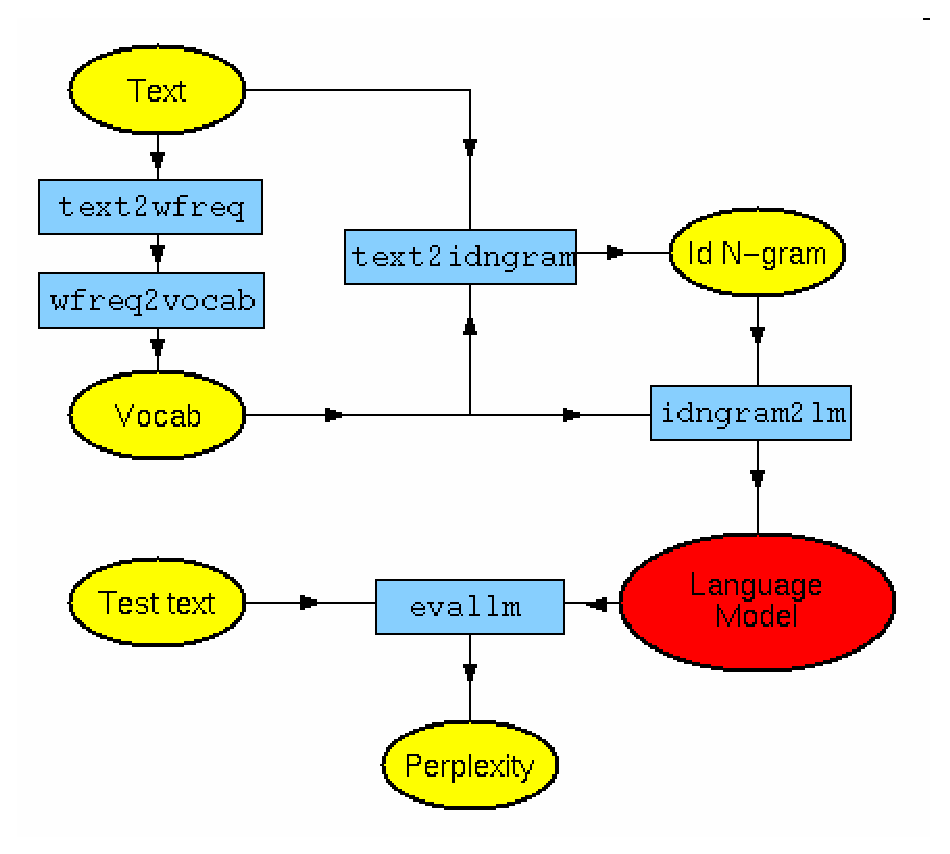
\includegraphics[width=\textwidth]{Bilder/toolkit.eps}
	%\caption{Eine Grafik}
	%\label{Bild}
	\end{minipage}
	% Auff�llen des Zwischenraums
	\hfill
	% minipage mit Grafik
	\begin{minipage}[b]{0.25\textwidth}
	% \textwidth bezieht sich nun auf die Minipage
 	Title\\
 	Job\\
 	Mitarbeit seit:1995\\	
	% \caption{Der Text}
	% \label{Text}
	\end{minipage}
	\hfill
	% minipage mit (Blind-)Text
	\begin{minipage}[b]{0.2\textwidth} 
	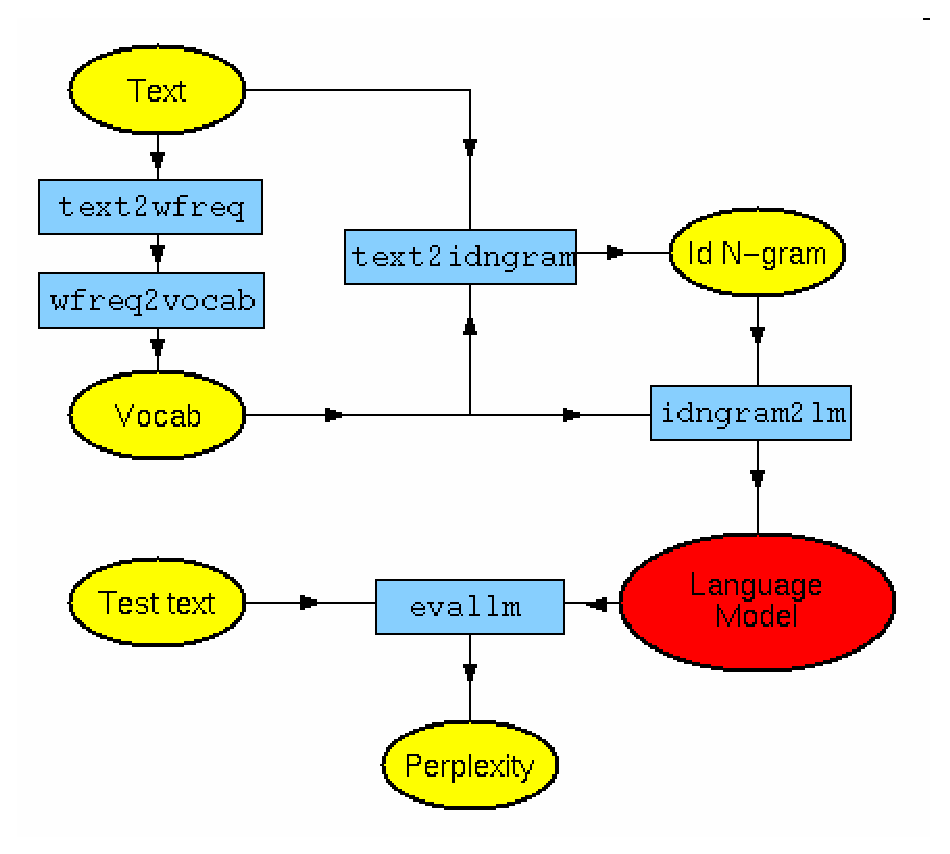
\includegraphics[width=\textwidth]{Bilder/toolkit.eps}
	%\caption{Eine Grafik}
	%\label{Bild}
	\end{minipage}
	% Auff�llen des Zwischenraums
	\hfill
	% minipage mit Grafik
	\begin{minipage}[b]{0.25\textwidth}
	% \textwidth bezieht sich nun auf die Minipage
 	Title\\
 	Job\\
 	Mitarbeit seit:1995\\	
	% \caption{Der Text}
	% \label{Text}
	\end{minipage}
% \caption{noch eine Caption}
\end{figure}

%Wissenschaftliche Mitarbeiter
%Scientific staff

\section*{Wissenschaftliche Mitarbeiter}


\chapter{Forschungsschwepunkte}
\echapter{RESEARCH}
%\LR{
		%\subsection{sub1 Parallel} 
		%\blindtext \blindtext \blindtext \blindtext
%		}{
		%\esubsection{sub2 Parallel}
		% \blindtext \blindtext \blindtext \blindtext
%}
\input{mainmatter/forschungsschwepunkte/regelung_von_PM}

\chapter{Labor}
\echapter{Labory}


\chapter{Lehrveranstaltungen}



\chapter{Kooperationen}

%\clearpage
%\bibliographystyle{get_deu_alphadin}							% default styles  get_alphadin} %     
%\bibliographystyle{alpha}
%\bibliographystyle{get_natdin}
%\bibliographystyle{get_eng_natdin}						% f? englische Texte
%\bibliographystyle{unsrtdin}
%\bibliographystyle{bib/IEEEtran}
%\bibliography{bib/Ref_xby}

\begin{figure}
  \figbicaption{fig:test}{Deutscher Titel}{English Title}
\end{figure}



\chapter{Title of first chapter}
\begin{refsection}
This is just filler text \parencite{massa}.
This is just filler text \parencite{augustine}.
This is just filler text \parencite{cotton}.
This is just filler text \parencite{hammond}.
\printbibliography[heading=subbibliography]
\end{refsection}

\chapter{Title of second chapter}
\begin{refsection}
This is just filler text \parencite{hammond}.
This is just filler text \parencite{massa}.
This is just filler text \parencite{cotton}.
This is just filler text \parencite{murray}.
\printbibliography[heading=subbibliography]
\end{refsection}

\chapter{Title of third chapter}
\begin{refsection}
This is just filler text \parencite{murray}.
This is just filler text \parencite{augustine}.
This is just filler text \parencite{cotton}.
This is just filler text \parencite{bertram}.
\printbibliography[heading=subbibliography]
\end{refsection}